\documentclass[../notes.tex]{subfiles}

\pagestyle{main}
\renewcommand{\chaptermark}[1]{\markboth{\chaptername\ \thechapter\ (#1)}{}}
\setcounter{chapter}{10}

\begin{document}




\chapter{Kinetics}
\section{Experimental Determination of Kinetic Isotope Effects}
\begin{itemize}
    \item \marginnote{11/12:}Lecture 18 recap.
    \begin{itemize}
        \item The physical basis and mechanistic interpretation of kinetic isotope effects.
        \item We also began discussing independent absolute rate measurement.
        \begin{itemize}
            \item Alex reviews the discussion associated with Figure \ref{fig:indepAbsRate}.
        \end{itemize}
    \end{itemize}
    \item Today: Experimental determination of KIEs.
    \begin{itemize}
        \item All of these examples are pulled from \textcite{bib:KIEexpt}.
    \end{itemize}
    \item Topic 2: Competition experiments.
    \begin{itemize}
        \item Can be run a couple of different ways.
        \item Most simple/natural progression from independent absolute rate measurement: Intermolecular competition.
        \item Then there is intramolecular competition.
    \end{itemize}
    \item Subtopic 2.1{}: Intermolecular competition.
    \begin{figure}[h!]
        \centering
        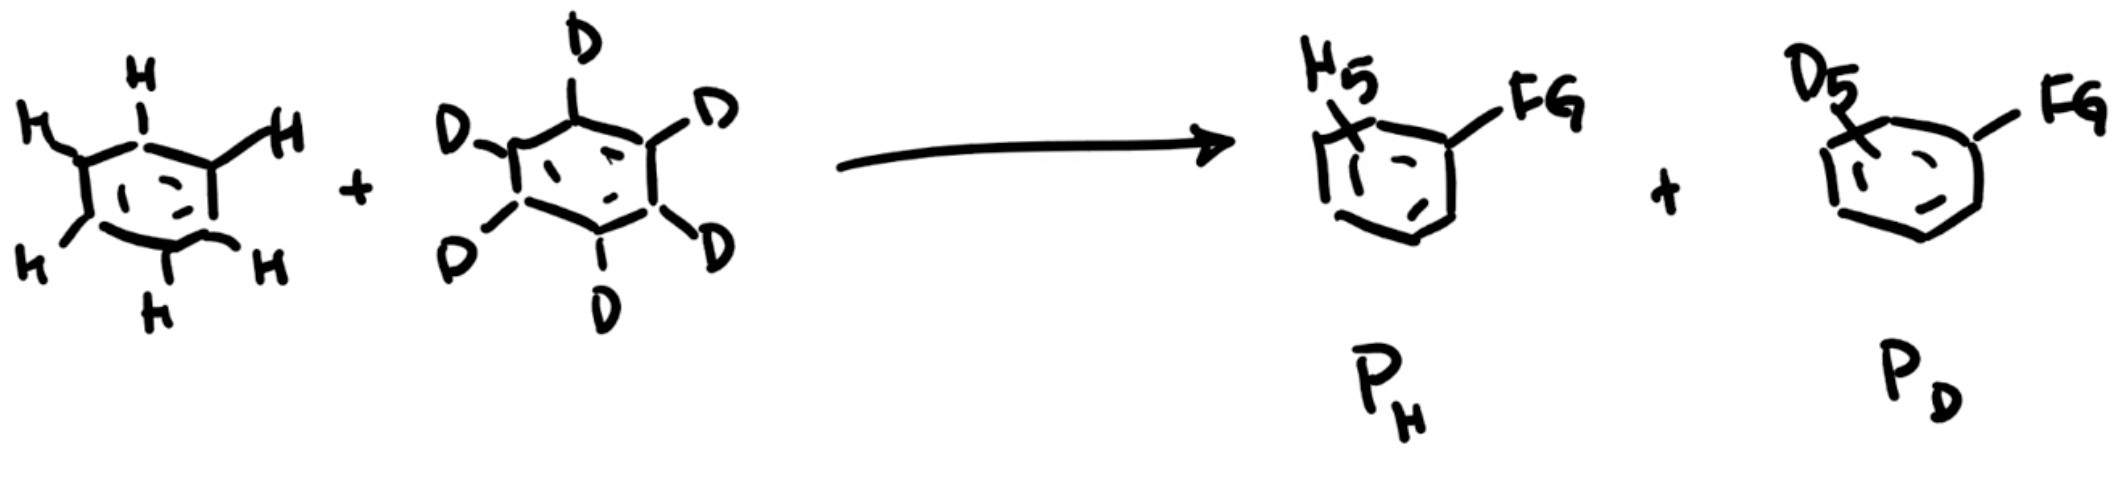
\includegraphics[width=0.7\linewidth]{compInter.png}
        \caption{Competition experiment (intermolecular).}
        \label{fig:compInter}
    \end{figure}
    \begin{itemize}
        \item Instead of running the protonated and deuterated substrates independently, throw them into the same pot at the same time.
        \item Take half an equivalent of the normal substrate and half an equivalent of the perdeuterated substrate.
        \begin{itemize}
            \item It doesn't have to be half an equivalent, but this makes the analysis easier.
            \item We also don't have to use the perdeuterated substrate, but it's often the easiest to make.
        \end{itemize}
        \item We then measure the ratio of undeuterated functionalized product vs. the deuterated functionalized product.
        \item We can then extract our KIE from the $\cnc{P_H}/\cnc{P_D}$ ratio.
        \item Caveat (this reaction is frequently run incorrectly in the literature!): We have to account for the fact that the concentrations of the starting materials are changing throughout.
        \begin{itemize}
            \item Indeed, the product and starting material are highly dependent on the conversion.
            \item The ratio of the products is equal to the ratio of the starting materials at high conversion.
            \item However, if we only run the reaction to low conversion, we can assume that the concentration of the starting material hasn't changed too much! Thus, the product ratio will reflect the actual KIE.
        \end{itemize}
        \item We can quantify products by NMR, LC-MS, GC-MS, etc.!
        \begin{itemize}
            \item So this reaction is experimentally simple to do because products are easy to quantify.
        \end{itemize}
        \item We can measure extremely small KIEs because our product-detection methods are so good!
        \item There is a contrasting paradigm in which we run to large conversions and characterize the remaining starting material ratio at the end.
        \begin{itemize}
            \item We'll get there later in the lecture.
        \end{itemize}
    \end{itemize}
    \item We have to apply a correction for conversion to extract the KIE at any conversion.
    \begin{itemize}
        \item Define
        \begin{align*}
            C &:= \frac{\cnc{P_H}}{\cnc[0]{SM_H}}&
            R &:= \left( \frac{\cnc{SM_D}}{\cnc{SM_H}} \right)_t&
            R_0 &:= \left( \frac{\cnc{SM_D}}{\cnc{SM_H}} \right)_0
        \end{align*}
        \begin{itemize}
            \item $C$ is the conversion.
            \begin{itemize}
                \item From the definition, we can tell that it is a number between 0 and 1.
            \end{itemize}
            \item $R$ gives the isotopic enrichment at any moment $t$.
            \item $R$ is the initial isotopic enrichment.
        \end{itemize}
        \item Thus, we can do some algebra to get a correction term that allows us to calculate the KIE from any time point.
        \begin{align*}
            \frac{R}{R_0} &= (1-C)^{k_{\ce{D}}/k_{\ce{H}}-1}\\
            \KIE = \frac{k_{\ce{H}}}{k_{\ce{D}}} &= \frac{\ln(1-C)}{\ln\left[ (1-C)\cdot\frac{R}{R_0} \right]}
        \end{align*}
        \item Takeaways.
        \begin{itemize}
            \item If we can extract both the conversion $C$ and isotopic composition $R/R_0$, we can extract the KIE accurately.
            \item If we run these reactions in replicates, we can get \emph{very} accurate KIEs!
        \end{itemize}
    \end{itemize}
    \item Note that at high conversions, the ratio of the deuterated to protonated starting materials goes to infinity. Symbolically,
    \begin{equation*}
        \frac{\cnc{SM_D}}{\cnc{SM_H}} \to \infty
    \end{equation*}
    \begin{itemize}
        \item Implication: As we get higher and higher conversions, we'll eventually reach a point where we only have a few molecules of starting material left, and almost all of them are the deuterated ones.
        \item This high-conversion exaggeration makes measurement easier.
        \item Indeed, at ultra-high conversions, we can get extremely accurate measurements for even very small KIEs!
    \end{itemize}
    \pagebreak
    \item Example: Kinetic isotope effects can narrow down which steps are or are not rate-determining.
    \begin{figure}[h!]
        \centering
        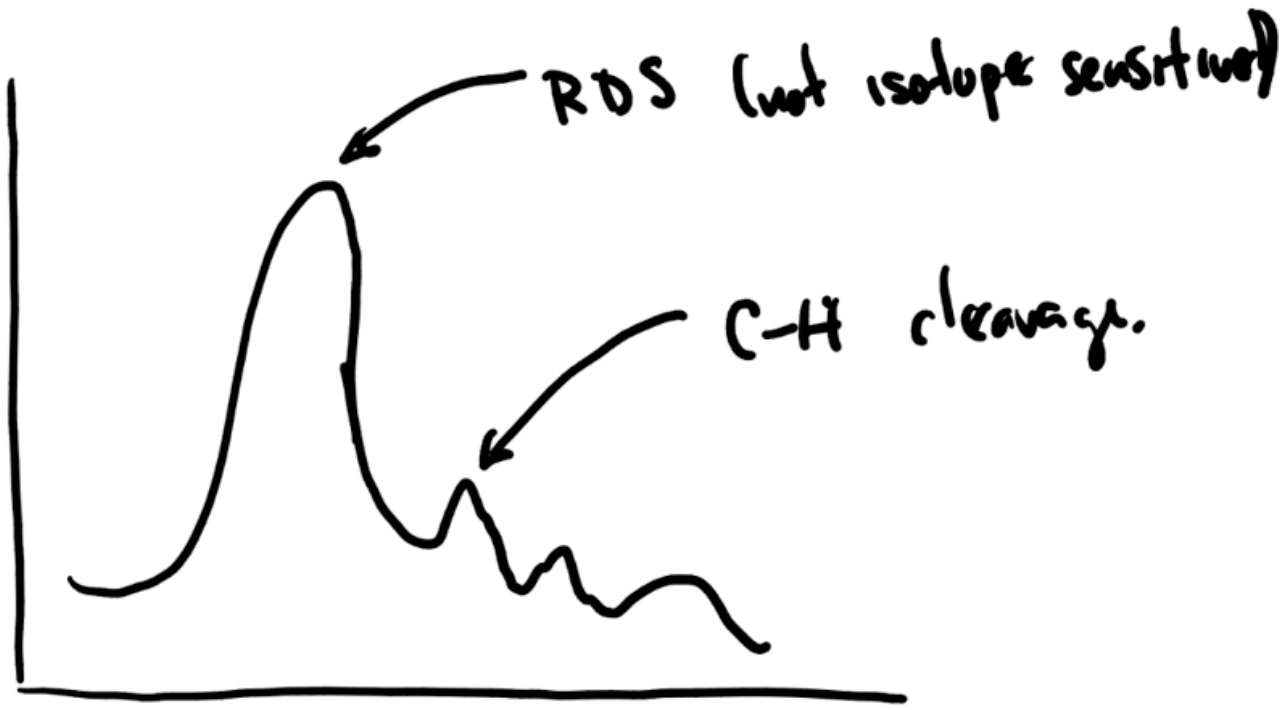
\includegraphics[width=0.4\linewidth]{PESpeakKIE.png}
        \caption{Assigning peaks on a potential energy surface by using kinetic isotope effects.}
        \label{fig:PESpeakKIE}
    \end{figure}
    \begin{itemize}
        \item Consider the reaction of \ce{H5}- and \ce{D5}-isotopologoues run both under a palladium-catalyzed arylation.
        \begin{center}
            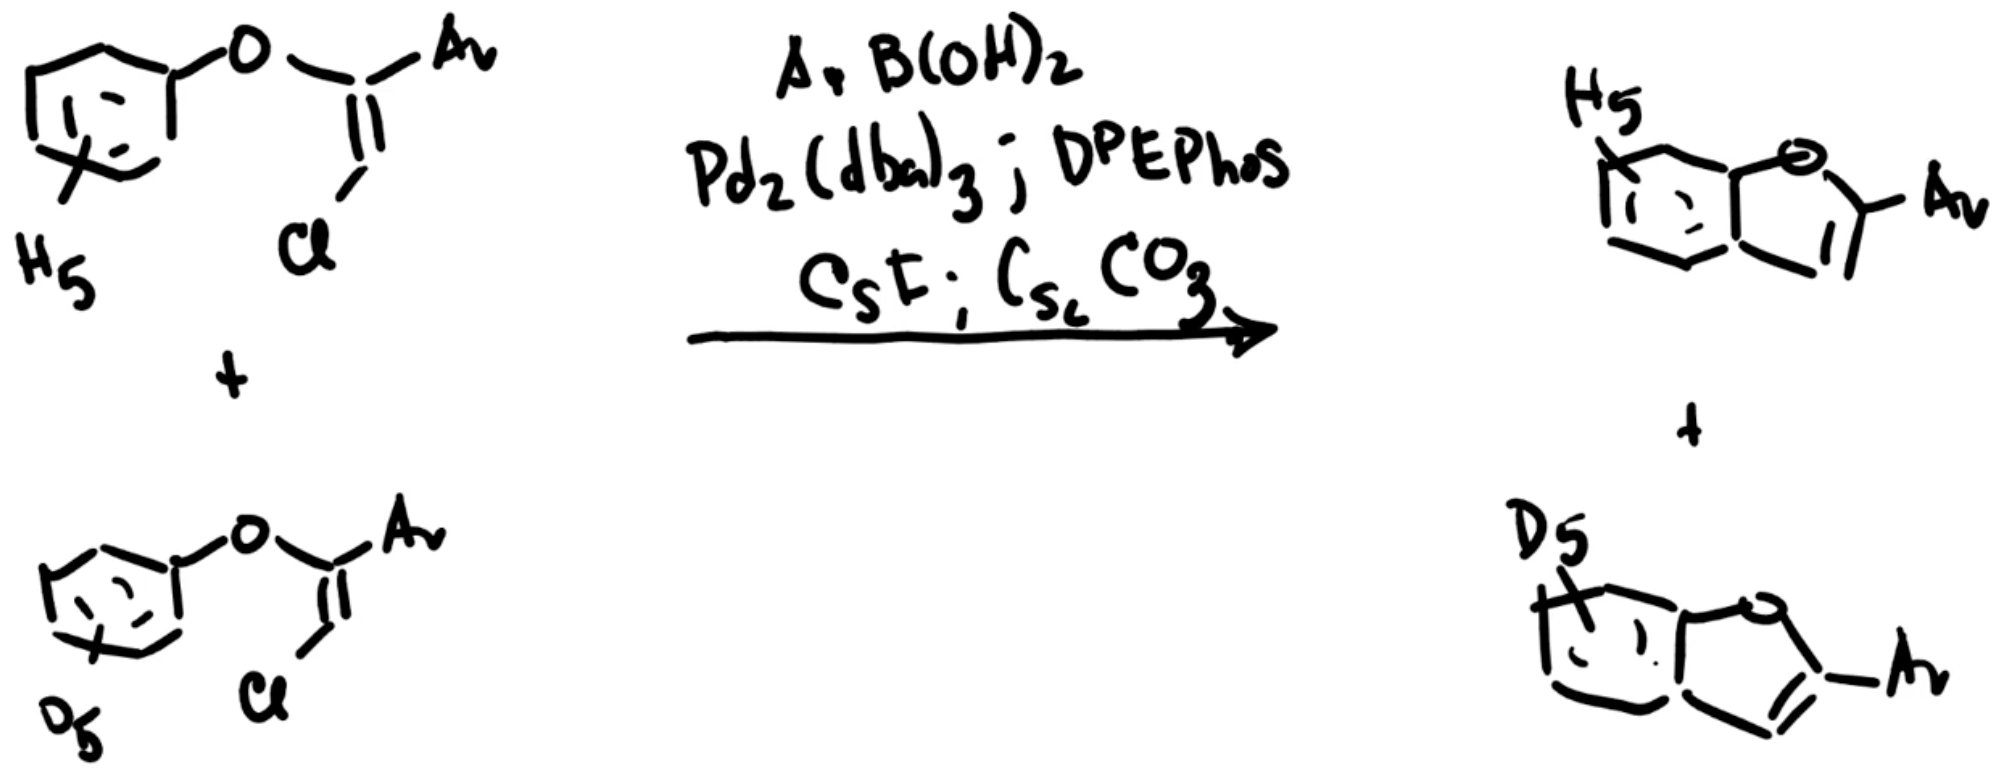
\includegraphics[width=0.7\linewidth]{PESpeakKIErxn.png}
        \end{center}
        \begin{itemize}
            \item Meant to be a Suzuki coupling (there's a boronic acid in there), but that ended up being irrelevant to the chemistry.
            \item In reality, the observed products are ring-closed.
        \end{itemize}
        \item We have \emph{no} intermolecular KIE (that is, $k_{\ce{H}}/k_{\ce{D}}=1.0$).
        \begin{itemize}
            \item This means that the rate of reaction is \emph{not} determined by the presence or absence of heavy isotopes.
            \item It follows that \ce{C-H/D} cleavage is \emph{not} the rate-determining step!
            % \item In contrast, if the big peak was rate-determining, we \emph{would} see an intermolecular KIE.
        \end{itemize}
        \item What does this mean in terms of the potential energy surface?
        \begin{itemize}
            \item It means that the largest peak (the RDS) does \emph{not} involve \ce{C-H/D} cleavage, but one of the other peaks could.
        \end{itemize}
        \item Reference: \textcite{bib:KIEexpt}.
    \end{itemize}
    \item Subtopic 2.2{}: Intramolecular competition.
    \item Example: Kinetic isotope effects can probe post-rate determining steps!
    \begin{itemize}
        \item Consider the same palladium-catalyzed arylation, but our substrate has one \ce{H} and one \ce{D} that can be cleaved.
        \begin{center}
            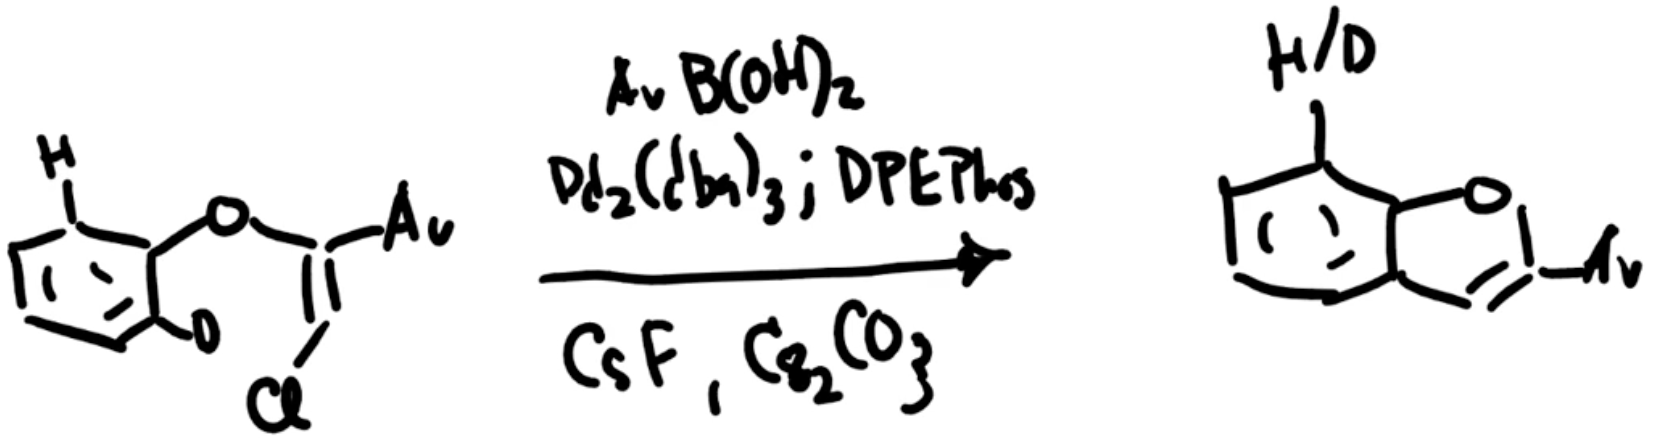
\includegraphics[width=0.57\linewidth]{KIEpostRDS.png}
        \end{center}
        \item Then you can quantify the amount of \ce{H} vs. \ce{D} at the \emph{ortho}-position in the product and extract an intramolecular KIE of 4.
        \item Thus, we have probed a post-rate determining step!
        \item In this case, oxidative addition to the $sp^2$-\ce{Cl} is believed to be rate-determining; but we can still use this intramolecular KIE to learn something useful for mechanistic analysis or further reaction development.
        \item Reference: \textcite{bib:KIEexpt}.
    \end{itemize}
    \item General structure of intramolecular KIEs.
    \begin{figure}[h!]
        \centering
        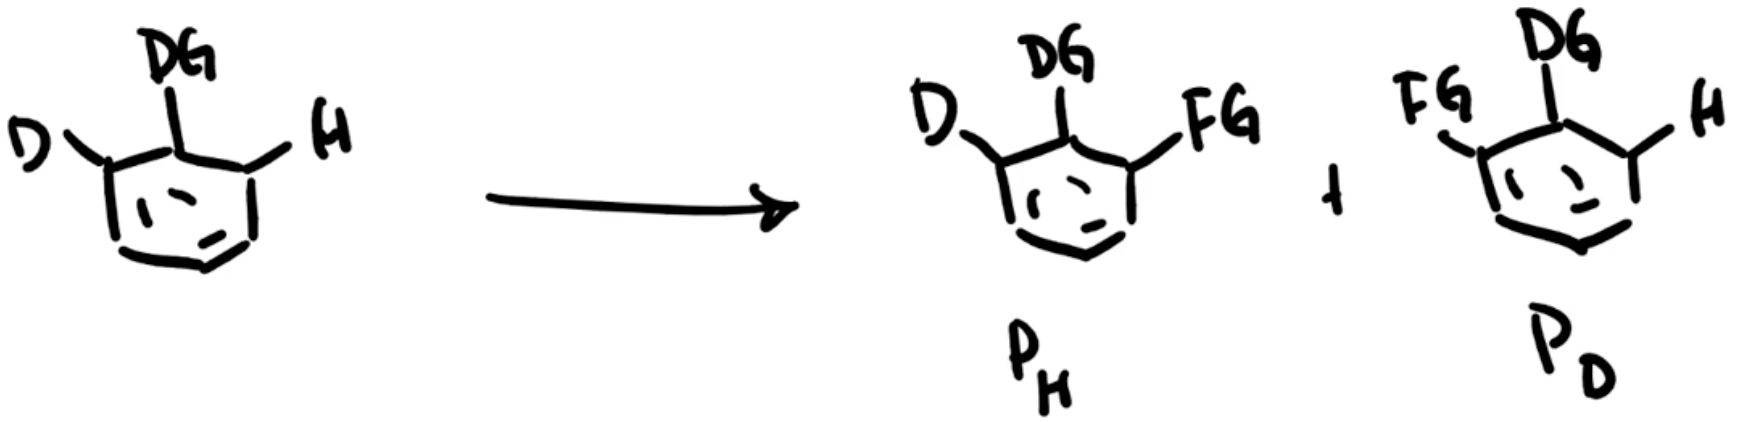
\includegraphics[width=0.55\linewidth]{compIntra.png}
        \caption{Competition experiment (intramolecular).}
        \label{fig:compIntra}
    \end{figure}
    \begin{itemize}
        \item We design a symmetric reactant with a donating group, an \ce{H} on one side, and a \ce{D} on the other side.
        \item Then the KIE can be rigorously extracted from
        \begin{equation*}
            \KIE = \frac{\cnc{P_H}}{\cnc{P_D}}
        \end{equation*}
        at \emph{any} conversion.
        \item We get to use any conversion because the reaction does \emph{not} enrich the isotopic composition.
        \begin{itemize}
            \item The (local) concentrations of \ce{H} and \ce{D} are fixed by the synthesis of the molecule!
        \end{itemize}
        \item This method gets us an "intrinsic" KIE, even for post-rate limiting steps.
    \end{itemize}
    \item To recap.
    \begin{itemize}
        \item Independent, intermolecular, and intramolecular.
        \item The results depend heavily on the conditions we use!
    \end{itemize}
    \item Topic 3: Heavy atom KIEs.
    \begin{itemize}
        \item We'll talk a bit more about the measurement of extremely small KIEs here.
        \item The most common heavy atoms to investigate are \ce{{}^12C}/\ce{{}^13C}.
        \begin{itemize}
            \item However, it can also be \ce{N}, \ce{O}, \ce{P}, \ce{Cl}, etc.
        \end{itemize}
        \item The magnitude tends to be small because of the smaller change in reduced mass (see Table \ref{tab:redMassBond}).
        \item Example: \ce{{}^12C}/\ce{{}^13C} KIEs tend to be 1.0-1.05.
        \begin{itemize}
            \item 1.05 is large, even --- by \ce{{}^12C}/\ce{{}^13C} standards, that is!
        \end{itemize}
        \item Because we have a small enrichment that is difficult to measure, it is very important to use sensitive methods.
        \item This also means that we can pretty much only measure \emph{primary} heavy atom KIEs; secondary heavy atom KIEs are usually too small to measure.
        \item Reference: \textcite{bib:HeavyAtomKIE}.
        \begin{itemize}
            \item Alex highly recommends to learn more about all aspects of heavy atom KIEs.
        \end{itemize}
    \end{itemize}
    \pagebreak
    \item We experimentally measure heavy atom KIEs using a series of experiments developed in the '90s.
    \item The most common is the Singleton Method for KIE determination.
    \begin{itemize}
        \item This is a determination done at the natural abundance of the various isotopologues.
    \end{itemize}
    \item Singleton's key insight \#1: \ce{{}^13C} is a naturally occurring (typically 1.1\% abundance) heavier isotope of \ce{{}^12C}.
    \begin{itemize}
        \item It follows that every molecule is already labeled with this heavy isotopologoue, and already labeled at every position.
    \end{itemize}
    \item Singleton's key insight \#2: \ce{{}^13C} can be measured via \ce{{}^13C} NMR for quantitation.
    \item Both of these insights are important because \ce{{}^13C} precursors are few and far between, and they're expensive! Labeling a certain position can be very difficult (and expensive).
    \item Singleton's key insight \#3: Recall that $R/R_0=(1-C)^{1/\KIE-1}$. As $C\to 1$, $R/R_0$ becomes very sensitive to the KIE.
    \begin{figure}[h!]
        \centering
        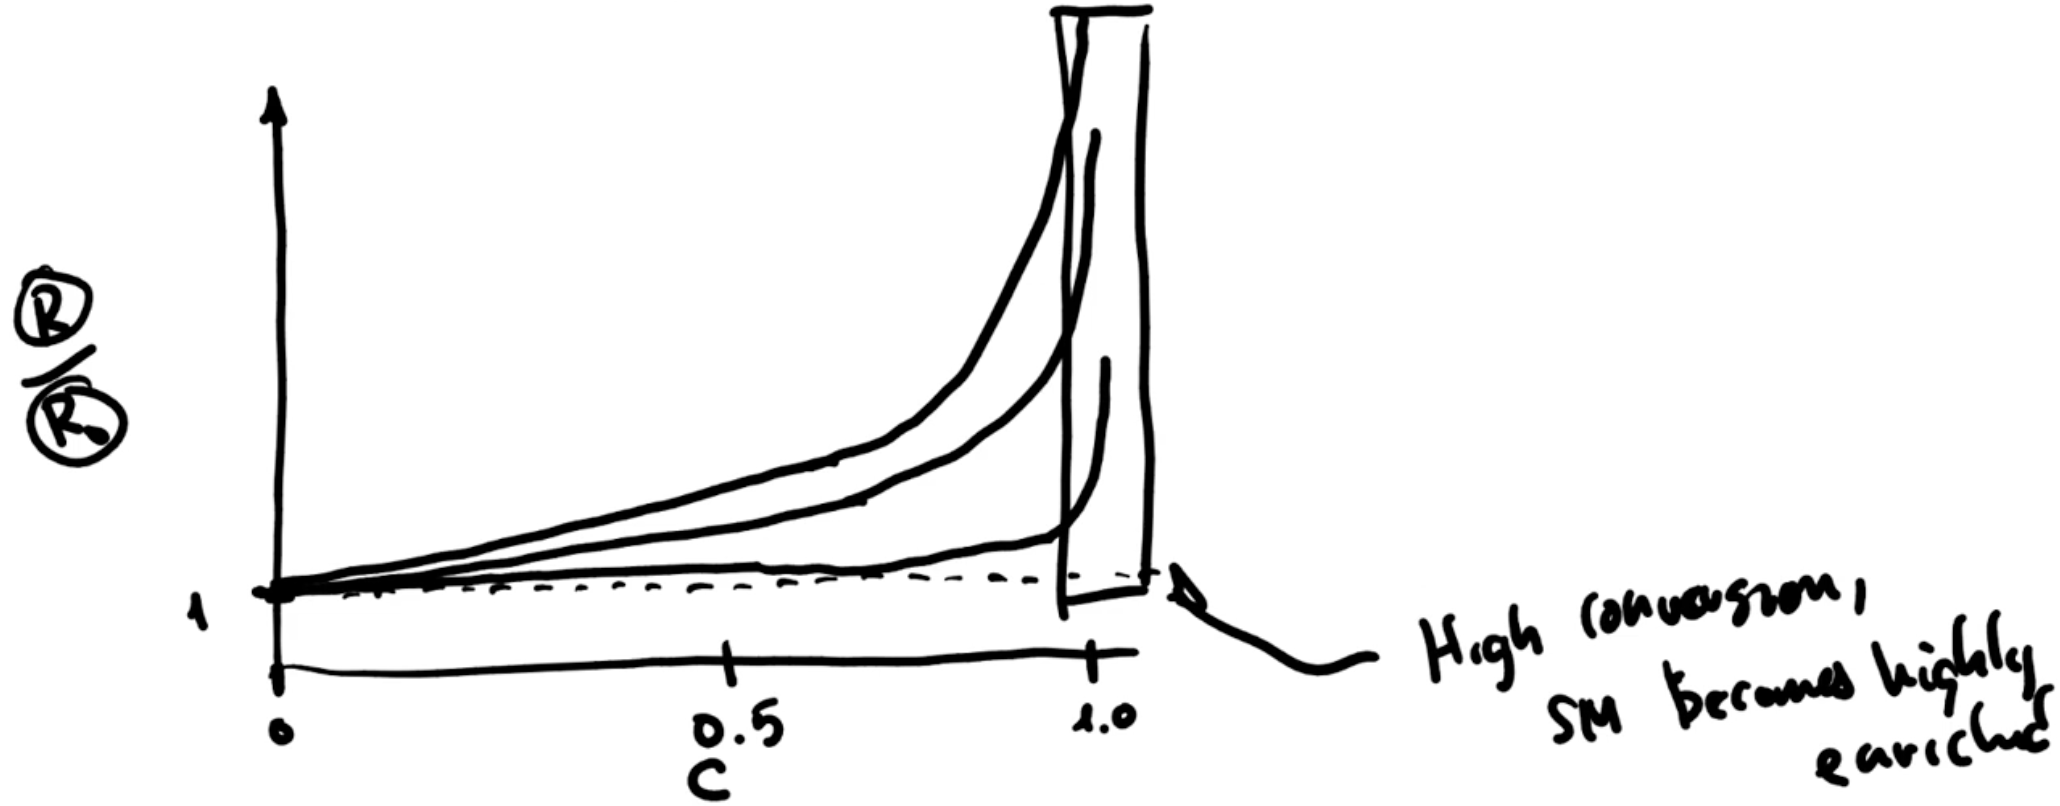
\includegraphics[width=0.7\linewidth]{isotopeEnrichHigh.png}
        \caption{Isotopic enrichment at high conversions.}
        \label{fig:isotopeEnrichHigh}
    \end{figure}
    \begin{itemize}
        \item We can visualize this relationship through a series of plots of $R/R_0$ vs. $C$.
        \begin{itemize}
            \item If we run a reaction with a KIE of 1.0, we'll have $R/R_0=1$ at any $C\in[0,1)$.
            \item If we run a reaction with even a KIE of 1.1, we'll get enrichment in the slower-reacting isotope later on that leads to larger KIEs!
        \end{itemize}
        \item Takeaway: At sufficiently high conversions, the starting material becomes highly enriched in the slow-reacting isotopologue.
    \end{itemize}
    \item Numerical data in support of Figure \ref{fig:isotopeEnrichHigh}.
    \begin{table}[h!]
        \centering
        \small
        \renewcommand{\arraystretch}{1.2}
        \begin{tabular}{cc}
            $\bm{C}$ & $\bm{R/R_0}$\\
            \hline
            $0.5$  & $1.03$\\
            $0.75$ & $1.07$\\
            $0.9$  & $1.12$\\
            $0.99$ & $1.25$\\
        \end{tabular}
        \caption{Isotopic enrichment at high conversions.}
        \label{tab:isotopeEnrichHigh}
    \end{table}
    \begin{itemize}
        \item Suppose the light over heavy rate constant ratio ($k_\text{L}/k_\text{H}$) is fixed equal to 1.05.
        \item We can get extremely accurate KIE measurements for even very such a small intrinsic KIEs, provided again that we run to sufficient converions.
    \end{itemize}
    \item Example: Measuring heavy atom kinetic isotope effects for an intermolecular reaction.
    \begin{figure}[H]
        \centering
        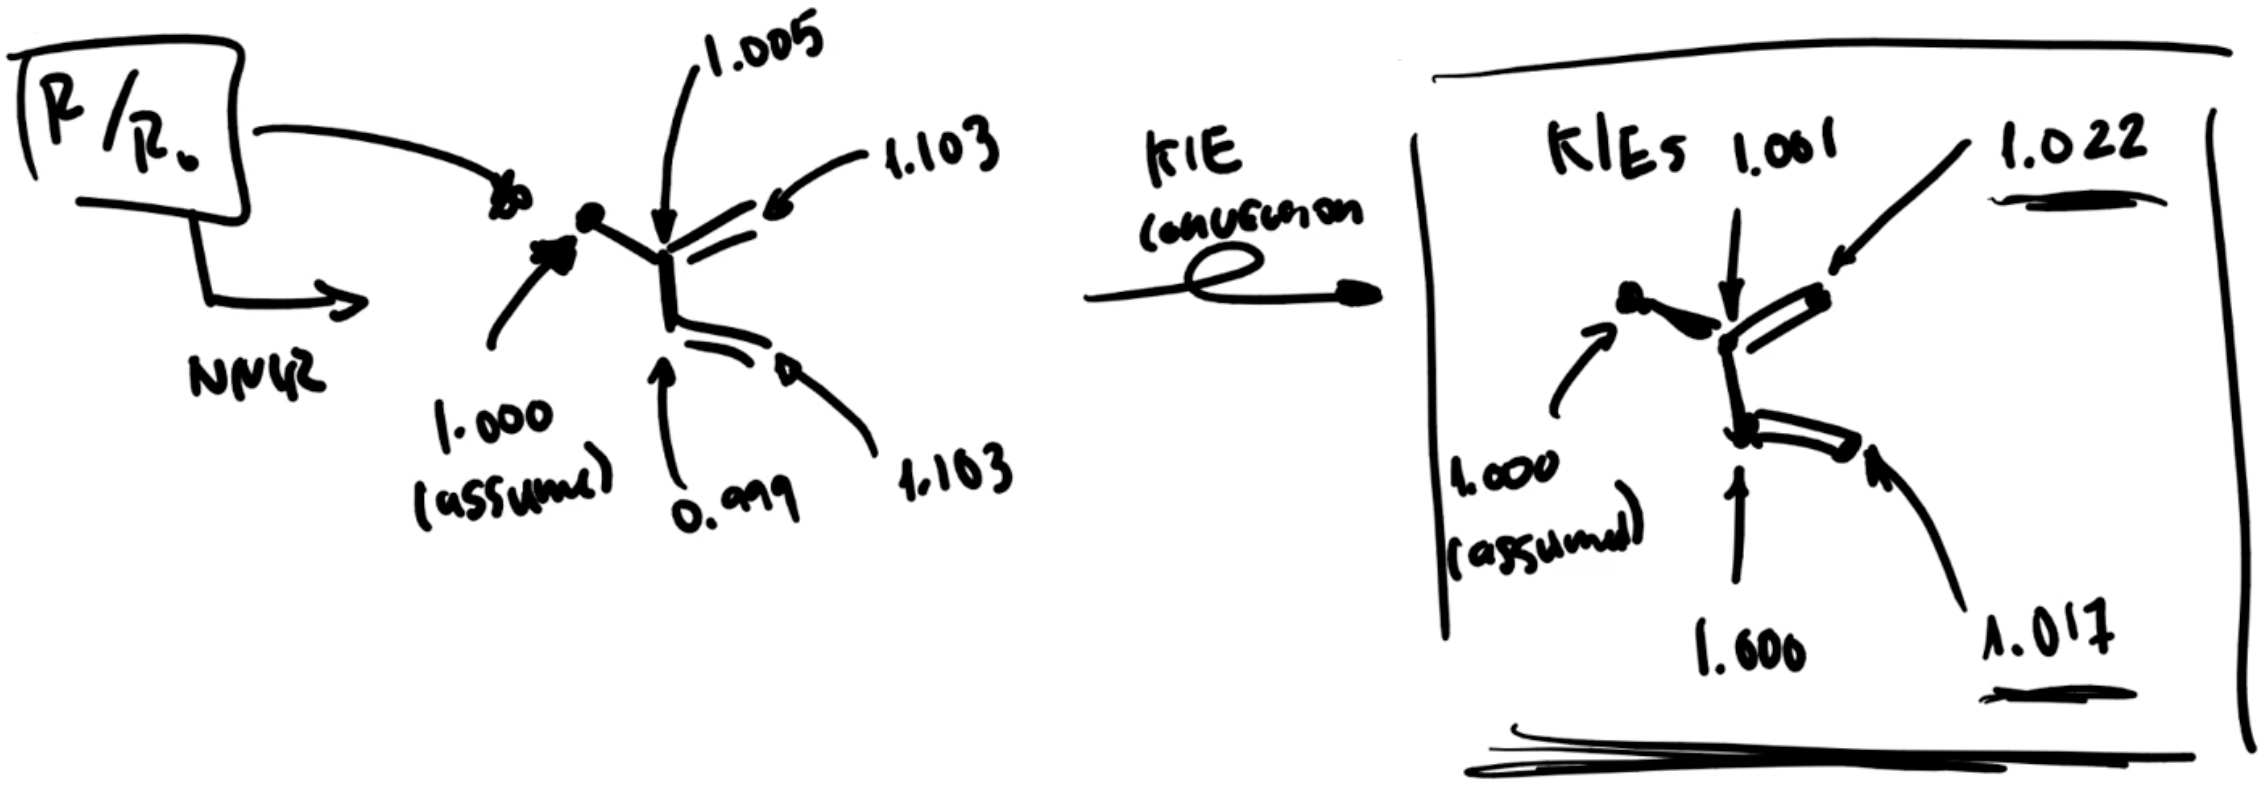
\includegraphics[width=0.75\linewidth]{SingletonInter.png}
        \caption{Singleton method for intermolecular heavy atom kinetic isotope effects.}
        \label{fig:SingletonInter}
    \end{figure}
    \begin{itemize}
        \item Consider the following Diels-Alder reaction.
        \begin{center}
            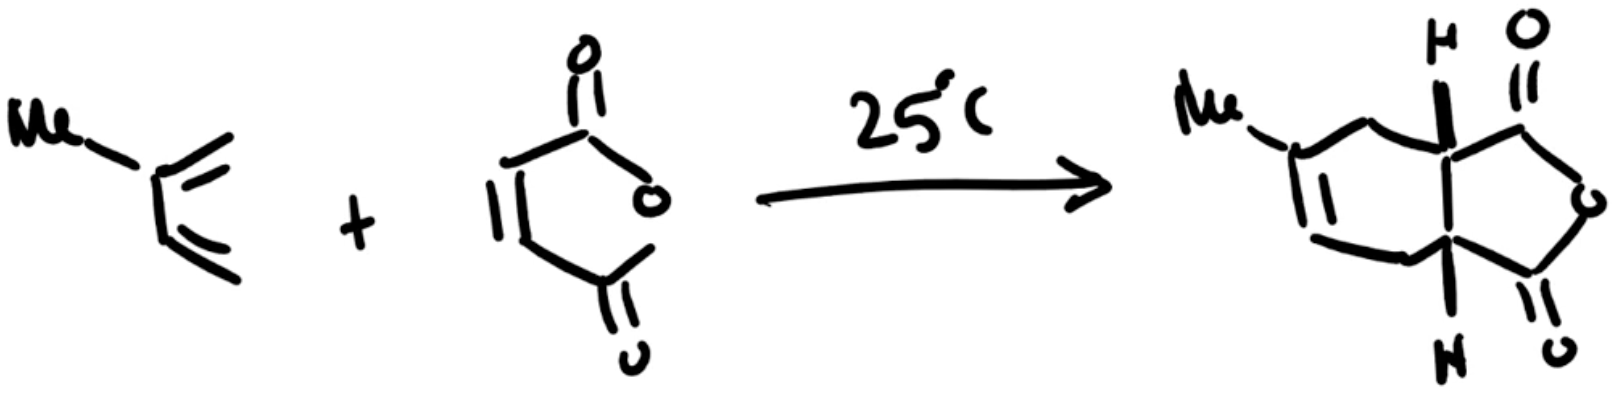
\includegraphics[width=0.55\linewidth]{SingletonInterRxn.png}
        \end{center}
        \item It was run to a conversion of 98.9\%.
        \item We then looked at the $R/R_0$ ratio in the diene starting material.
        \begin{itemize}
            \item We do this with NMR measurements.
            \item Assume that there is a position in the molecule (e.g., the remote methyl) that is not isotopically sensitive, and hence has $\KIE=1.000$.
            \begin{itemize}
                \item If we pick our site well, this is a reasonable assumption.
            \end{itemize}
            \item We then measure the raw integrals at the other sites.
            \item Take these integrals, put them back into the equation we derived previously to obtain the KIE ratio.
            \begin{itemize}
                \item Example:
                \begin{equation*}
                    \KIE = \frac{k_{\ce{H}}}{k_{\ce{D}}} = \frac{\ln(1-0.989)}{\ln\left[ (1-0.989)\cdot\frac{1.103}{1.000} \right]} = 1.022
                \end{equation*}
            \end{itemize}
        \end{itemize}
        \item Conclusion: The biggest KIEs are at the terminal methyl groups (as expected from the Woodward-Hoffmann rules; this is another confirmation!), and we get a slight improvement in rate on the side near the methyl group.
        \begin{itemize}
            \item It would probably be prohibitive to label each position in the diene, but just a good mathematical knowledge of conversions gets us everything we need.
        \end{itemize}
        \item Reference: \textcite{bib:SingletonInter}.
    \end{itemize}
    \item Limitations of the Singleton method.
    \begin{itemize}
        \item We need a large amount of sample.
        \begin{itemize}
            \item This is because we're running the reaction to high conversion, but need to isolate the starting material.
            \item So in order to get accurate NMRs, we need sufficiently high concentrations of the sample.
            \item We can run Diels-Alders on nearly mole scales, and potentially isolate grams; that's why the previous example worked.
        \end{itemize}
        \item The reaction must be irreversible.
        \begin{itemize}
            \item It it isn't, we're going to get equilibrium isotope effects mixed in.
        \end{itemize}
        \item The results can be difficult to interpret.
        \begin{itemize}
            \item Any individual number might not be too helpful, but with modern quantum mechanical calculations, we can match our results to a DFT-computed potential energy surface!
            \item This will show that one pathway has a better experimental match with KIEs.
            \item This is good evidence for a mechanistic course!!
        \end{itemize}
        \item Natural abundance experiments can be run in both inter- and intramolecular modes.
    \end{itemize}
    \item Example: Measuring heavy atom kinetic isotope effects (aka "natural abundance experiments") in an intramolecular mode.
    \begin{figure}[h!]
        \centering
        \begin{subfigure}[b]{0.45\linewidth}
            \centering
            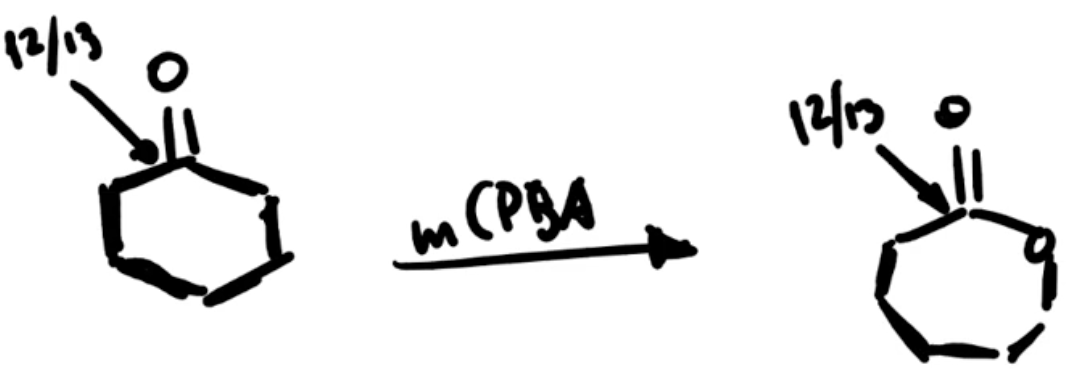
\includegraphics[width=0.8\linewidth]{SingletonIntraa.png}
            \caption{Relevant labeling for intermolecular data.}
            \label{fig:SingletonIntraa}
        \end{subfigure}
        \begin{subfigure}[b]{0.45\linewidth}
            \centering
            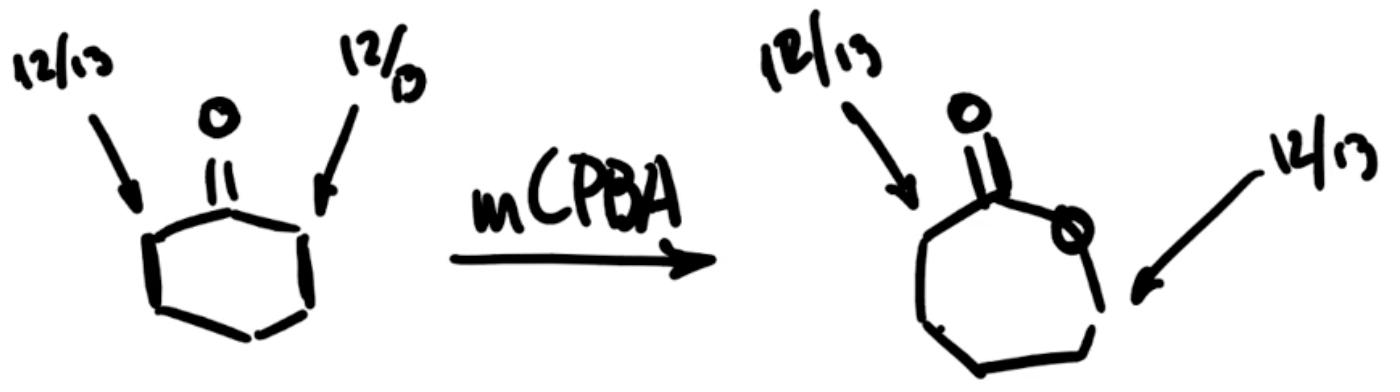
\includegraphics[width=0.99\linewidth]{SingletonIntrab.png}
            \caption{Relevant labeling for intramolecular data.}
            \label{fig:SingletonIntrab}
        \end{subfigure}\\[2em]
        \begin{subfigure}[b]{0.3\linewidth}
            \centering
            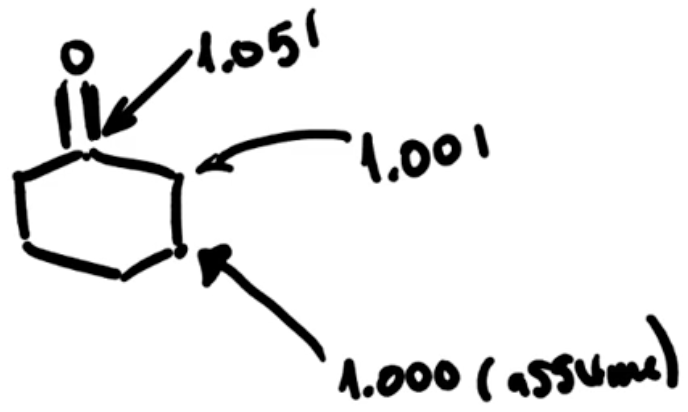
\includegraphics[width=0.75\linewidth]{SingletonIntrac.png}
            \caption{Intermolecular KIEs.}
            \label{fig:SingletonIntrac}
        \end{subfigure}
        \begin{subfigure}[b]{0.3\linewidth}
            \centering
            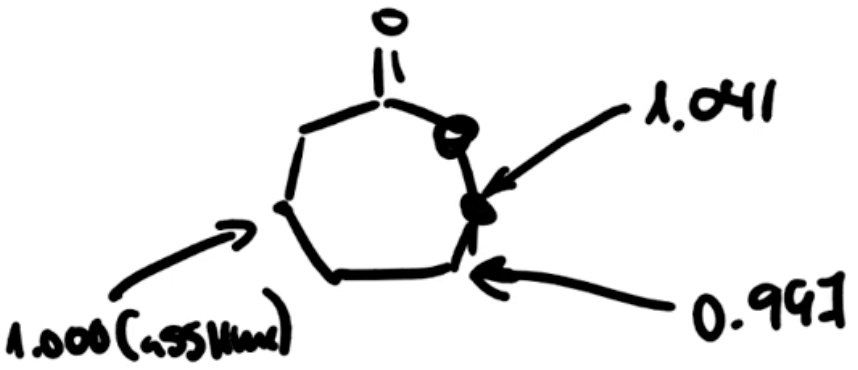
\includegraphics[width=0.95\linewidth]{SingletonIntrad.png}
            \caption{Intramolecular KIEs.}
            \label{fig:SingletonIntrad}
        \end{subfigure}
        \caption{Singleton method for intramolecular heavy atom kinetic isotope effects.}
        \label{fig:SingletonIntra}
    \end{figure}
    \begin{itemize}
        \item Consider the Baeyer-Villiger reaction.
        \begin{center}
            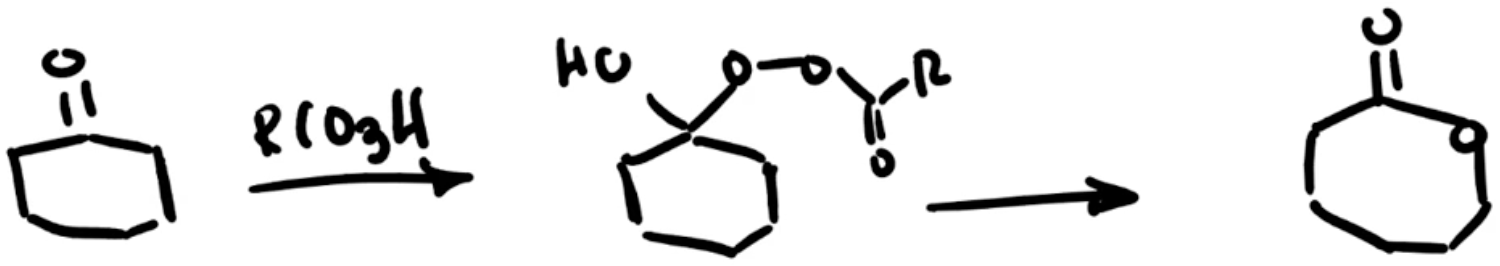
\includegraphics[width=0.6\linewidth]{SingletonIntraRxn.png}
        \end{center}
        \begin{itemize}
            \item A ketone reacts with a peracid.
            \item The mechanism is believed to proceed through a hemiacetal, followed by ring expansion to the lactone.
        \end{itemize}
        \item So we have a two-step mechanism.
        \begin{itemize}
            \item We can probe the first step with natural abundance KIE to determine whether or not hemiacetal formation is rate-determining.
            \item Simultaneously (in the same pot/set of experiments), we can probe the second step with an intramolecular heavy atom KIE.
        \end{itemize}
        \item Intermolecular variant: Consider the labeling at the \emph{ipso}-position.
        \begin{itemize}
            \item Run this reaction to a known conversion, quantitate that conversion well, isolate the starting material, and quantitate its \ce{{}^12C}/\ce{{}^13C} well (using, e.g, mass spec).
            \item Isotopic enrichment of the starting material, here, is conversion-dependent (because it's affiliated with the RDS).
            \item We assume that the $\beta$-position has an isotopic enrichment of 1.000.
            \item The resultant significant isotopic fractionation of the starting material ($\KIE=1.051$) implies that the initial conversion of the ketone to the acetal is rate-determining.
        \end{itemize}
        \pagebreak
        \item Intramolecular variant: Consider the labeling at the $\alpha$-positions.
        \begin{itemize}
            \item Isotopic enrichment of the product, here, is conversion-independent (because it's post-RDS).
            \item We assume that the $\beta$-position has an isotopic enrichment of 1.000.
            \item The resultant significant isotopic fractionation of the product ($\KIE=1.041$) implies that the migration step occurs after the RDS, and involves the $\alpha$-position.
        \end{itemize}
        \item It is somewhat counterintiutive that hemiacetal formation (typically fast) would be rate-limiting!
        \item Reference: \textcite{bib:SingletonIntra}.
    \end{itemize}
    \item Takeaways from today.
    \begin{itemize}
        \item We get deep and important information about reaction courses, rate-determining steps, etc. from isotope effects.
    \end{itemize}
    \item Next time: Kinetics and kinetic rate laws.
\end{itemize}




\end{document}